%%%%%%%%%%%%%%%%%%%%%%%%%%%%%%%%%%%%%%%%%%%%%%
% Header
\documentclass[12pt]{article}
\usepackage[english]{babel}
\usepackage[utf8x]{inputenc}
\usepackage{graphicx}
\usepackage{amsthm}
\usepackage{amsmath}
\PassOptionsToPackage{hyphens}{url}\usepackage{hyperref}
\usepackage{geometry}
\usepackage{fullpage}
\usepackage{float}
\usepackage[lastexercise]{exercise}

\setlength{\parindent}{0cm}

\renewcommand{\ExerciseHeader}{\large\textbf{\ExerciseName~\ExerciseHeaderNB} - \textbf{\ExerciseTitle}\medskip}

\renewcommand{\ExePartHeader}{\medskip\textbf{\ExePartName\ExePartHeaderNB\ExePartHeaderTitle\medskip}}

\begin{document}
%%%%%%%%%%%%%%%%%%%%%%%%%%%%%%%%%%%%%%%%%%%%%%
\subsubsection*{EMAT10007 -- Introduction to Computer Programming}
\subsection*{\Large Exercises -- Week 10. Classes and External Libraries}

\section*{Classes:}

\begin{Exercise}[title=Supermarkets with Classes]

Recall the Supermarkets exercise from Week 5. Now we will be attempting something similar but with classes.
    \begin{center}
     \begin{tabular}{||c c c c||} 
     \hline
     Item & Stock & Cost & Price \\ [0.5ex] 
     \hline\hline
     Apple & 35 & 0.1 & 0.2 \\ 
     \hline
     Avocado & 10 & 0.7 & 1 \\
     \hline
     Bananas & 0 & 0.08 & 0.15 \\
     \hline
     Gai Lan & 10 & 0.75 & 1.3 \\
     \hline
     Carrots & 15 & 0.05 & 0.1 \\
     \hline
     Pomelo & 2 & 1.2 & 1.5 \\
     \hline
     Tomatoes & 20 & 0.35 & 0.50 \\
     \hline
     Pineapple & 0 & 0.8 & 1.25 \\ [1ex] 
     \hline
    \end{tabular}
    \end{center}
    \Question{Create a class called {\tt Item}. Give it the following constructor (or initialiser):
    
    \vspace{0.5em}
    {\tt def \_\_init\_\_(self):}\\
    {\tt \hspace*{2em} print("Creating a new item")}
    \vspace{0.5em}
    
    Now create an instance of the class {\tt Item} called {\tt Apple}. What happens?
    }
    \Question{Now change the constructor like so:
    
    \vspace{0.5em}
    {\tt def \_\_init\_\_(self, Name):}\\
    {\tt \hspace*{2em} print("Creating a new item:", Name)}\\
    {\tt \hspace*{2em} self.Name = Name}
    \vspace{0.5em}
    
    Now our {\tt Item} class has a name attribute. Recreate the {\tt Apple} instance assigning it the name {\tt "Apple"}. What happens now? Call {\tt print(Apple.Name)}.
    }
    \Question{Add these additional attributes to the {\tt Item} class: {\tt Stock, Cost, Price}.
    }
    \Question{Recreate the {\tt Apple} instance with the parameters given in the table.}
    \Question{Add the method {\tt PrintItemInfo(self)} to the {\tt Item} class. It should print out all the information about the item.
    
    Call {\tt Apple.PrintItemInfo()} from the main program.
    }
    \Question{Create a list called {\tt ItemInfoList} and add to it an instance of the {\tt Item} class for every item in the table.}
    \Question{Add another method {\tt CheckStock(self, Threshold)} which returns {\tt True} if the items stock is greater than the threshold and {\tt False} is it is less than or equal to it. How would you change this so that the default value for {\tt Threshold} is 0?}
    \Question{Write a loop in the main program which checks all items in {\tt ItemInfoList} and prints out any items which have a stock less than or equal to two.}
    \Question{Add the method {\tt SellItem(self, Quantity)} to the {\tt Item} class. If there is enough stock, it should print the price of the item and reduce the stock by the quantity.}
    \Question{Refer back to the Week 5 exercise sheet. Answer those questions again using the {\tt Item} class.}
\end{Exercise}

\begin{Exercise}[title={Supermarket with Classes and Inheritance}]
    \begin{center}
     \begin{tabular}{||c c c c c||} 
     \hline
     Item & Stock & Cost & Price & Restriction \\ [0.5ex] 
     \hline\hline
     Scissors & 4 & 3.5 & 4 & 18\\ 
     \hline
     Paracetamol & 10 & 0.4 & 0.8 & 16 \\ 
     \hline
     Cider & 15 & 2 & 3.5 & 18 \\ [1ex] 
     \hline
    \end{tabular}
    \end{center}
    \Question{Add a new class called {\tt RestrictedItems} which \emph{inherits} from the {\tt Item} class. Note the constructor should first call the constructor of the {\tt Item} class, passing in the {\tt Name}, {\tt Stock}, {\tt Cost}, and {\tt Price} arguments. Then it should add the {\tt Restriction} variable as an attribute of the new class.
    }
    \Question{Add items in the above to the {\tt ItemInfoList} as instances of the {\tt RestrictedItems} class.
    }
    \Question{Override the {\tt PrintItemInfo()} method of the {\tt Item} class so that it also now prints the restriction.
    }
    \Question{Override the {\tt SellItem()} method of the {\tt Item} class so that it now prompts for a check of the buyer's age before continuing.
    }
\end{Exercise}

\section*{External libraries:}

\begin{Exercise}[title=Numpy and Matplotlib: Simple Projectile]

Suppose we want to plot the motion of a ball after it has been kicked. We can use the following equations to calculate the displacement in $x$ and $y$ at time $t$ as:
\begin{equation*}
    x = v_0 t \cos\theta \qquad \text{and} \qquad
    y = v_0 t \sin\theta - 0.5gt^2,
\end{equation*}
where $v_0$ is the initial velocity, $\theta$ is the initial launch angle and $g$ is the gravitational acceleration constant ($g=9.81ms^{-2}$) (see the figure).

\begin{center}
   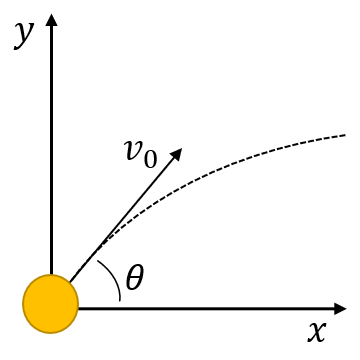
\includegraphics{projectileImage.png}
\end{center}

\Question{First {\tt import} the {\tt numpy} and {\tt matplotlib.pyplot} external libraries or \emph{modules}. Recall that when importing a module we can it an alias using {\tt import module as m}. Common aliases are {\tt np} for {\tt numpy} and {\tt plt} for {\tt matplotlib.pyplot}.}
\Question{Define {\tt GRAVITY=9.81} as a constant.}
\Question{Create the function {\tt CalcDisplacement} which calculates the displacement in $x$ and $y$ when $t=1$. It should accept the arguments {\tt InitalVelocity}, {\tt Angle}, {\tt Time}. It should return the displacement as a vector {\tt numpy} array object.

\textbf{Hint:} Use the {\tt numpy} versions of $\cos$ and $\sin$. The {\tt np.array()} function takes an iterable and converts it into a {\tt numpy} array object. To create a vector we simply create a one-dimensional array. Just like vectors these can be represented both vertically and horizontally. (\url{https://docs.scipy.org/doc/numpy/reference/generated/numpy.array.html})
}
\Question{Call the function with the parameters $v_0 = 30ms^2$, $\theta = \frac{\pi}{3}$rad and $t=2s$. What values do you get?}
\Question{Create a function called {\tt CalcNewPosition} which adds the result of the {\tt Displacement} function to the ball's {\tt InitialPosition} which should be a {np.array} object.}
\Question{What is the ball's new position at $t=2s$ if its initial position was $(x_0, y_0) = (10, 0)$?}
\Question{Calculate the Euclidean distance between these two points using the {\tt np.linalg.norm()} function. 

\textbf{Hint:} Recall that the Euclidean distance is the same as the $2$-norm for vectors. \url{https://docs.scipy.org/doc/numpy/reference/generated/numpy.linalg.norm.html}
}
\Question{Now we want to find the path of the ball as it travels. Write the following {\tt for} loop which calculates the positions of the ball as $t$ changes from $0$ to $5$ with $(x_0, y_0) = (0, 0)$, $v_0=30$ and $\theta=\frac{\pi}{3}$. It stores these positions in a two-dimensional matrix.
    
    \vspace{0.5em}
    {\tt \# Create an array of 100 evenly spaced values from 0 to 10}\\
    {\tt TimePoints = np.linspace(0, 10, num=100)}\\
    {\tt \# Initialise an empty array with shape 2x100}\\
    {\tt Positions = np.empty((2, 100))}\\
    {\tt for i, Time in enumerate(TimePoints):}\\
    {\tt \hspace*{2em} NewPosition = CalcNewPosition(<?>)}\\
    {\tt \hspace*{2em} Positions[:, i] = NewPosition \# <??>}
    \vspace{0.5em}

Fill in with {\tt <?>} blank with the correct inputs to match your {\tt CalcNewPosition} function. (N.B. There should be four of them.)

\Question{What does the line {\tt Positions[:, i] = NewPosition} do? How would you fill in the blank comment {\tt <??>}?}}
\Question{Now that we have all the positions we can plot them using the {\tt plot} function from {\tt matplotlib.pyplot}. Create a plot showing the projectile of the ball by following the example given here: \url{https://matplotlib.org/3.1.1/gallery/lines_bars_and_markers/simple_plot.html#sphx-glr-gallery-lines-bars-and-markers-simple-plot-py}.}

\textbf{Hint:} Remember that the first row of {\tt Positions} are all the $x$ values and the second row all the $y$ values.
\Question{What happens if we calculate the positions of the ball as $t$ changes from $0$ to $10$? You should see that the ball's $y$-position becomes negative. This is because we are not enforcing the ground at $y=0$.

We can use the function {\tt np.where()} to check for when the ball hits the ground. Once the ball has hit the ground it should stay on the ground (assuming no bounce).
Add the following line:

    \vspace{0.5em}
    {\tt Positions[1, :] = np.where(<?>, <??>, <???>)}.
    \vspace{0.5em}

Fill in the blanks such that:

\begin{itemize}
    \item {\tt <?>} is a condition checking whether {\tt Positions[1,:]} is less than 0.
    \item {\tt <??>} is the new value for when the condition is true.
    \item {\tt <???>} leaves the value unchanged if the condition is false.
\end{itemize}

\textbf{Hint:} Remember the documentation is there to help.
}
\Question{Earlier we calculated the Euclidean distance between the ball's initial position and its position for some time $t$. Create a plot showing how this distance changes over time.  
}
\Question{In this exercise, we have taken a simple mechanics problem and solved it using the external libraries {\tt numpy} and {\tt matplotlib}. You can do the same for a wide variety of problems. There are also many ways we could extend this:
    \begin{itemize}
        \item Use the {\tt np.max()} function to find the maximum height the ball reaches and plot this.
        \item Show how the parabola that the projectile changes depending on the initial launch angle.
        \item Add this to a Tkinter GUI where the user can enter parameter values and generate the projectile plot.
    \end{itemize}
    }
\end{Exercise}

\begin{Exercise}[title=PyGame: Making an `enemy' class.]

	The goal of this exercise is to write a class that produces the behaviour of an enemy sprite, which will wander randomly and will steal a random amount of gold bricks from any player it touches. Start by downloading the {\tt PyGame\_base\_code.py} program from Blackboard, as we will use this as our base.\\
	
	\textbf{Note:} When overwriting an attribute or class method from a parent class (i.e. the one being inherrited from) you must use \textbf{exactly} the same name, including case. For example, this is why the {\tt update()} method begins with a lower case letter, and is not in keeping with our normal naming convention of {\tt Upper CamelCase}.  
	
	\Question{Write a class called {\tt Enemy} that inherits from the {\tt pygame.sprite.Sprite} class. We want to create a class that is very similar in structure to the {\tt Player} class i.e.\ creating a square sprite, colouring it, initialising its speed variables to $0$ etc.}

    \Question{Start by implementing an {\tt \_\_init\_\_()} method that follows the general layout from the {\tt Player} class:

		\begin{itemize}
			\item Add a new argument to the {\tt \_\_init\_\_()} method to set the size of the enemy sprite as well as the starting x and y coordinates.

			\item Make the default colour of the enemy sprite be {\tt RED} (you will have to define a new colour at the top of the code).

			\item Set the {\tt self.Size} variable to store the size argument.

			\item The rest should be kept the same.
		\end{itemize}
	}

	\Question{Implement the same {\tt update()} method, as the game requires that all sprites implement an update method.}

    \Question{Next, we're going to add a new method to our {\tt Enemy} class which, given an {\tt EnemySpeed} and the length and width of the window, has our enemy move randomly within the window:

		\begin{enumerate}
	    \item Because we want our Enemy to change direction at random times, rather than every time we loop through the main code, we need to begin by creating a {\tt Delay} variable inside the Enemy class (but not within the new method -- usually at the top underneath the class definition) and setting it to $0$.

		\item Create a method with the following signature:
			
			\vspace{0.5em}
			{\tt MoveRandomly(self, Speed, XLimit, YLimit):}
			\vspace{0.5em}
			
			where {\tt Speed} will be the speed at which the enemy moves. {\tt XLimit} and {\tt YLimit} will be the window's width and height, to act as bounds within which our enemy will move.

		\item Then, {\tt IF Delay == 0}, we will set a random direction for our enemy:

			\begin{itemize}
				\item For each possible compass direction e.g. a random direction in
				
				\begin{equation*}
				    [\mathbf{``N", ``NE", ``E", ``SE", ``S", ``SW", ``W", ``NW"}]
				\end{equation*}
				
				pick a random direction in the list and have the sprite change its {\tt ChangeX} and {\tt ChangeY} values to move in that direction based on its speed.

				\item Then, after picking an initial direction to travel in (as delay is set to $0$ when the sprite is created), we need to pick a random value for delay e.g. a value between $5$ and $100$.
			\end{itemize}

		\item {\tt ELSE}

			\begin{itemize}
				\item decrement the {\tt Delay} variable by $1$
			\end{itemize}
			
    	\item Then we need to ``bounce'' the enemy. This can be tricky but the gist is that:

			\begin{itemize}
				\item If the enemy position is too far left ($< 0$) or too far right ($>$ {\tt XLimit}), reverse the x-direction e.g.\\
				{\tt ChangeX = ChangeX * -1}

				\item Similarly, if the enemy position is too high ($< 0$) or too low ($>$ {\tt YLimit}), reverse the y-direction e.g.\\
				{\tt ChangeY = ChangeY * -1}

				\item To be more precise, you will need to adjust the conditions checking the {\tt XLimit} and {\tt YLimit} to account for the size of the sprite.
			\end{itemize}
	    \end{enumerate}}
	\Question{Create a new instance of the {\tt Enemy} class, assigning it to a variable called {\tt Enemy1} and giving it a starting position and size e.g. $(400, 400)$ and $30$. Then add the enemy to the {\tt AllSpritesList}, so that it will be drawn on-screen with the other sprites.}

	\Question{After the input loop, but \textbf{before} {\tt AllSpritesList.update()}, add a call to our Enemy's {\tt MoveRandomly()} method, passing in the window's dimensions as follows:
		
		\vspace{0.5em}
		{\tt Enemy1.MoveRandomly(EnemySpeed, 800, 600)}
		\vspace{0.5em}
		
		where {\tt EnemySpeed} should probably be a lower value than the {\tt SPEED} variable we set for the players e.g.\ $5$. We could increase the difficulty later by increasing the {\tt EnemySpeed}.}
\end{Exercise}

\begin{Exercise}[title=PyGame: Collision detection for the enemy class.]
    
    	Now that we have our enemy moving in random directions, we need to have the {\tt Enemy} sprite detect when it touches a player, and then reduce the player's score by stealing a random amount of gold bricks. We can use the existing collision detection code as a basis for having the enemy detect when it touches a player.
	
	\Question{First, we will need to add the players to a new sprite group, called {\tt PlayerList}, so that we can detect collisions for \textbf{only} the players, and not the gold bars.}

	\Question{Then, add both {\tt Player1} and {\tt Player2} to our {\tt PlayerList}.}

	\Question{Next, in the same location as we detect if players are touching the gold bars, we need to check if {\tt Enemy1} is touching any players in {\tt PlayerList}, and store the result in a list called {\tt EnemyHitList}.}

	\Question{Finally, we can set an amount to be stolen as {\tt StealAmount}, and loop through the list. For each player in the list, reduce their score by {\tt StealAmount}. You should also check that if {\tt player.score < 0}, that you set their score to $0$ so that they cannot possess a negative score.}
	\Question{(*) If you wanted, you could even implement a score for the enemy sprite and display the total amount of stolen gold bricks between the scores of Player1 and Player2.}
\end{Exercise}


\end{document}